\chapter{Extract Transform Load}\label{etl}
This project will require the extraction, manipulation and processing of a data source from one data model to another. This process is commonly known as Extract Transform Load (ETL). Section \ref{etlprocess} discusses each stage involved in the ETL procedure followed by section \ref{etltool} which examines the ETL implementation methodology and its relevance to this project. 

\section{Process}\label{etlprocess}
A basic definition of the Extract Transform Load (ETL) process is pulling data from one database, refactoring the composition of the data and putting the data into another database. While the name ETL implies there are 3 main categorisation stages - extract, transform, load - the procedure in its entirety is a much broader and expansive process which encompass these stages. Despite this the procedure is split in to these three stages. Figure \ref{fig:etl} illustrates the ETL process with data coming from a source; a file or database management system for example then being transformed in to the required format for a successful load. \begin{figure}[h]\begin{center}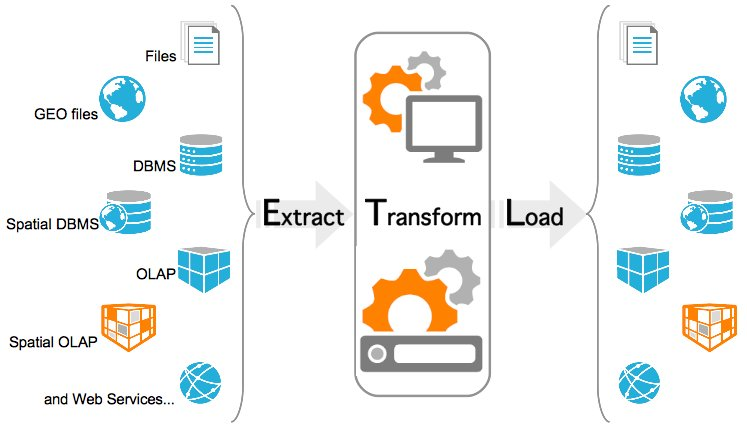
\includegraphics[width=0.8\linewidth]{images/etl.jpg}\caption{ETL process}\label{fig:etl}\end{center}\end{figure}

\subsection{Extract}
Extract is the first step in the ETL procedure in which data is read from a source system, usually a database but not restricted to, and makes it available for processing. The main objective of the extract stage is to retrieve all the required data from a source system using as little resources as possible \cite{etlref1}. It is common for data to be extracted from source systems with different organisations and formats to that of the target system. The extract stage provides an opportunity to \textit{cleanse} the data from the source system as often there will be redundant or irrelevant data which is not required.

\subsection{Transform}
Transform is where the extracted data is manipulated from its previous state and converted into a target system format. The step involves the application of a set of rules or functions to transform the data from the source to the target. As well as the applied rules and functions the transformation step is responsible for the validation of records ensuring unacceptable records are removed accordingly. ``The most common processes used for transformation are conversion, clearing the duplicates, standardizing, filtering, sorting, translating and looking up or verifying if the data sources are inconsistent." \cite{etlref2}.

\subsection{Load}
Load completes the three step procedure and is where data is written into the target system. There are multiple ways in which data is loaded into a system using the ELT methodology. One of which and the most obvious is to physically insert the data. For example if the target repository is a SQL database insert the data as a new row using the relevant \textit{Insert} statement. An alternative to loading the process manually is that some ETL tool implementations have the capability to ``...link the extraction, transformation, and loading processes for each record from the source." \cite{etlref2}. Depending on the technique applied the load step of the process can become the most time consuming.